\subsection{Geometry Based Methods} \todo{Skriv om PDR.}
In this section, we will describe two different techniques to compute a position of an object geometrically.

\subsubsection{Triangulation} \label{sec:triangulation}
Triangulation is described in \cite{Triangulation}.

Triangulation is based on measuring angles of known points in space. The receiving object measures the angles towards the signals transmitted to it, known as \gls{aoa}. Different techniques are applied to measure AOA, one of the common being using an array of directionally placed sensors. Another approach is to use two sensors placed in parallel. The time point at which the sensors receive the signal is likely to be different and can be used to compute the angle of the received signal.

As seen in \textbf{\autoref{fig:AOAAngle}}, having two sensors with distance $r$ apart and distance $\Delta l$, the angle $\alpha$ can be calculated with $\alpha = \arcsin (\frac{\Delta l}{r})$, where $\Delta l$ can be represented as $\Delta t$, which can be determined by \gls{tdoa} measurement.

\begin{figure}[H]
    \centering
    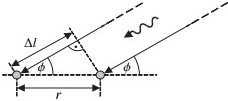
\includegraphics[scale=1.0]{Images/ProblemAnalysis/AOA_fig.jpg}
    \caption{Depiction of sensor placement to enable signal angle measurement\cite{Triangulation}.}
    \label{fig:AOAAngle}
\end{figure}

The disadvantage of triangulation is that it requires the mentioned additional sensors in order to calculate this angle.

\subsubsection{Trilateration} \label{sec:trilateration}
Trilateration is described in \cite{Triangulation}.

In trilateration, the position of an object is calculated by solving three equations of circles representing the range from the beacon to the object. This is illustrated in \textbf{\autoref{fig:trilateration}}.
By letting the beacons be denoted as $a$, $b$ and $c$, and the object to locate $m$, we can solve the following equations for $x_m$ and $ym$, where $l$ is the radius of each circle:

\begin{equation} \label{eq:CirclesCalculation1}
    (x_m - x_a)^2 + (y_m - y_a)^2 = l_{am}^2
\end{equation}
\vspace{-3mm}
\begin{equation} \label{eq:CirclesCalculation2}
    (x_m - x_b)^2 + (y_m - y_b)^2 = l_{bm}^2
\end{equation}
\vspace{-3mm}
\begin{equation} \label{eq:CirclesCalculation3}
    (x_m - x_c)^2 + (y_m - y_c)^2 = l_{cm}^2
\end{equation}

\begin{figure}[H]
    \centering
    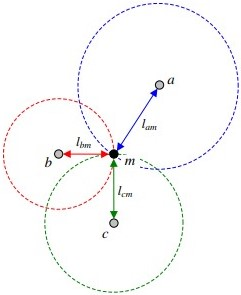
\includegraphics[scale=0.8]{Images/ProblemAnalysis/trilateration.jpg}
    \caption{Illustration of locating an object using three beacons with the use of trilateration\cite{Triangulation}.}
    \label{fig:trilateration}
\end{figure}

\subsubsection{Centroid}
How centroid location algorithms are used in locating objects is described in \cite{5759777}.

Centroid is, like triangulation and trilateration, based on beacons and the locations of the beacons. The goal is to provide a location estimate of an object given a vector of \gls{rssi} values. There exists two algorithms to locate an object: a range-based, which uses several distance to beacon estimations obtained from \gls{rss} measurements, and a range-free, which determines a location without distance estimations. These two algorithms are identified as WCL and REWL, respectively.

WCL approximates the location of an object by calculating the centroid of the coordinates of the beacons that are in range. WCL makes use of the equation seen in \textbf{\autoref{eq:WCLApproximaion}} to estimate the location of an object, where $a_i$ is the coordinates of a beacon and $\hat{d}_i$ is the distance between the object and beacon $a_i$, estimated using \gls{rss} values. Furthermore, $g > 0$ is an exponent that determines the weight of the contributions from each beacon. Using this equation, the distance from the object to each of the beacons within range is taken into account.

\begin{equation} \label{eq:WCLApproximaion}
    \hat{p} = \frac{\sum_{i = 1}^{n} (\hat{d}_i^{-g} * a_i)}{\sum_{i = 1}^{n} (\hat{d}_i^{-g})}
\end{equation}

In the estimation of the position of an object using REWL, REWL favors the beacons transmitting with higher \gls{rssi} values, since those are likely to be closer to the object. A weighting factor $\lambda$ is used in \textbf{\autoref{eq:REWLApproximation}}, where $RSS_{max}$ is the maximum value of all of the \gls{rss} measures measured by the object. The values of the weighting function $\lambda$ usually span from $0.1$ to $0.1$.

\begin{equation} \label{eq:REWLApproximation}
    \hat{p} = \frac{\sum_{i = 1}^{n} [(1 - \lambda)^{RSS_{max} - RSS_{i}} * a_i]}{\sum_{i = 1}^{n} (1 - \lambda)^{RSS_{max} - RSS_{i}}}
\end{equation}

\subsection{IMU positioning} \label{sec:IMUPositioning} % Kan måske stå et andet sted, så det kan skrives mere abstrakt her.
How positions are calculated with he use of IMU is described in \cite{IMUPositioning}.

As mentioned in \textbf{\autoref{sec:actuator_sensor}}, IMU consists of an accelerometer, a gyroscope and a magnetometer, and makes use of these to compute a position. Using IMU positioning, one can compute a position by the displacement of an initial position. This is also the disadvantage of IMU positioning, since an initial position is required.

To compute a position using IMU positioning, one starts by using the Euler method to compute the velocity of the moving object given data from the accelerometer. The equation for this computation is seen in \textbf{\autoref{eq:EulerAcceleration}}, where, $\Delta$ denotes the difference, $a$ is the accelerometer data and $t$ is time. Therefore, $\Delta v$ is the difference between two velocities. Now, \textbf{\autoref{eq:EulerDisplacement}} can be used to compute the displacement from the initial position. Combining \textbf{\autoref{eq:EulerAcceleration}} and \textbf{\autoref{eq:EulerDisplacement}} and the current acceleration reading, $a$, we can compute the total displacement using \textbf{\autoref{eq:TotalDisplacement}}.

\begin{equation} \label{eq:EulerAcceleration}
    v_n = \sum^{n} \Delta v_i = \sum^{n} a_i \Delta t_i = a_n \Delta t_n + \sum^{n - 1} a_i \Delta t_i = a_n \Delta t_n + v_{n - 1}
\end{equation}

\begin{equation} \label{eq:EulerDisplacement}
    s = \sum^{n} \Delta s_i = \sum^{n} v_i \Delta t_i = v_n \Delta t_n + \sum^{n - 1} v_i \Delta t_i = v_n \Delta t_n + s_{n - 1}
\end{equation}

\begin{equation} \label{eq:TotalDisplacement}
    s = v \Delta t + s_{n - 1} = (a \Delta t + v_{n - 1}) \Delta t + s_{n - 1} = s_{n - 1} + v_{n - 1} \Delta t + \frac{a}{2} \Delta^2 t
\end{equation}

The position of the object can be represented as in \textbf{\autoref{eq:IMUPosition}}, where $\begin{bmatrix}p_{x_{i}} \\ p_{y_{i}}\end{bmatrix}$ is the initial position.

\begin{equation} \label{eq:IMUPosition}
    \begin{bmatrix}p_{x} \\ p_{y}\end{bmatrix} = \begin{bmatrix}p_{x_{i}} \\ p_{y_{i}}\end{bmatrix} + \begin{bmatrix}s_{x} \\ s_{y}\end{bmatrix} = \begin{bmatrix}p_{x - 1} \\ p_{y - 1}\end{bmatrix} + \begin{bmatrix}\Delta s_{x} \\ \Delta s_{y}\end{bmatrix}
\end{equation}

\subsubsection{\gls{pdr}}
The \gls{pdr} method is described in \cite{HybridPositioningPaper}.

\gls{pdr} tracking is based on step detection algorithms, step length estimations $l_t$ and heading measurements $\theta_t$, all used to solve the problem defined in \textbf{\autoref{eq:pdr_x}} and \textbf{\autoref{eq:pdr_y}}.

\begin{equation} \label{eq:pdr_x}
    x_t = x_{t - 1} + l_t\cos(\theta_t)
\end{equation}

\begin{equation} \label{eq:pdr_y}
    y_t = y_{t - 1} + l_t\sin(\theta_t)
\end{equation}

The basic idea behind step detection is to use accelerometer measurements to observe increase and decrease in acceleration.
Pre-processing of accelerometer measurements is needed, since the measurements can be too noisy. This pre-processing consists of a gravity factor used in a high-pass filter and a low-pass filter, as defined in \textbf{\autoref{eq:high_pass_filter}} and \textbf{\autoref{eq:low_pass_filter_acc}} using the acceleration measurements data, defined in \textbf{\autoref{eq:acc_measurements}}. A high-pass filter is applied to remove a gravity factor, and low-pass filter acceleration is used to <SOMETHING>, as defined in \textbf{\autoref{eq:low_pass_filter_acc}}.

\begin{equation} \label{eq:acc_measurements}
    a_{eff, t} = \sqrt{a_{x, t}^2 + a_{y, t}^2 + a_{z, t}^2}
\end{equation}

\begin{equation} \label{eq:high_pass_filter} \todo{Inkludér ligning for high-pass filter, ikke bare denne gravitational factor som bruges i high-pass filter. Vi mangler i hvertfald noget af referere til med a_{HPF} i low-pass filter.}
    g_{z, t} = \alpha g_{z, t - 1} + (1 - \alpha) a_{eff, t}
\end{equation}

\begin{equation} \label{eq:low_pass_filter_acc}
    a_{LPF}[i] = \frac{1}{m} \sum_{j = \frac{-(m - 1)}{2}}^{\frac{m - 1}{2}} a_{HPF}[i + j]
\end{equation}

The gravity factor in \textbf{\autoref{eq:high_pass_filter}} is subtracted from the acceleration measurements data, where $\alpha$ is a constant, typically defined as $0.9$. The low-pass filter defined in \textbf{\autoref{eq:low_pass_filter_acc}} is stored for use in the step detection algorithm, where $m$ is a moving average filter, set to $10$.
Regarding the step detection algorithm, two methods can be used: the zero-crossing method and the peak detection method, both of which are out of scope for this section. \todo{Vælg én af disse metoder og beskriv den.}

For step length estimation, there exists two methods: static and dynamic. The static method assumes a person is walking at a constant velocity, whereas the dynamic method makes use of an accelerator for dynamic estimation. Weinberg is one method for dynamic step length estimation, which is defined as in \textbf{\autoref{eq:weinberg}}

\begin{equation} \label{eq:weinberg}
    l = k \sqrt[4]{a_{LPF, peak} - a_{LPF, valley}}
\end{equation}

In \textbf{\autoref{eq:weinberg}}, $k$ is a constant factor, for example, $0.5$, $a_{LPF, peak}$ is the maximum acceleration in the z-axis and $a_{LPF, valley}$ is the minimum acceleration.

Heading estimation is accomplished with the use of the IMU.